\documentclass{article}
\usepackage[utf8]{inputenc}
\usepackage{graphicx}
\usepackage{booktabs}
\usepackage{float}
\graphicspath{ {./metrics/fold_0/} }
\graphicspath{ {./metrics/fold_1/} }
\graphicspath{ {./metrics/fold_2/} }
\title{Results: bert-base-uncased-baseline-lr-[0.00005|0.00001|0.000001]}
\author{Nadia Sheikh}
\date{2022-07-25}
\begin{document}
\maketitle
\section{Configurations}
\subsection{Run Configuration}
\begin{tabular}{ll}
\toprule
{} &                                                  0 \\
\midrule
experiment\_identifier &                          llm-baseline-[bert|sbert] \\
run\_identifier        &  bert-base-uncased-baseline-lr-[0.00005|0.00001... \\
config\_file\_path      &  /home/nadia/Documents/CLaC-Lab/ctre/cnc-task-3... \\
\bottomrule
\end{tabular}

\subsection{Data Configuration}
\begin{tabular}{ll}
\toprule
{} &                                                  0 \\
\midrule
data\_utility\_cls        &                                      cnc\_utilities \\
dataset\_cls             &                                   CNCTask3aDataset \\
nos\_of\_folds            &                                                  3 \\
trn\_data\_path           &    /cnc-task-3/script-development/data/CSV-Output/ \\
tst\_data\_path           &  /home/nadia/Documents/CLaC-Lab/ctre/cnc-task-3... \\
base\_output\_folder\_path &             /cnc-task-3/script-development/output/ \\
config\_file\_path        &  /home/nadia/Documents/CLaC-Lab/ctre/cnc-task-3... \\
\bottomrule
\end{tabular}

\subsection{Preprocessing Configuration}
\begin{tabular}{ll}
\toprule
{} &                                                  0 \\
\midrule
collate\_fn\_name   &                                       LLMCollateFn \\
llm\_name          &                                  bert-base-uncased \\
connl\_folder\_path &  /home/nadia/Documents/CLaC-Lab/ctre/cnc-task-3... \\
max\_nos\_tokens    &                                                 84 \\
token\_sep         &                                               True \\
config\_file\_path  &  /home/nadia/Documents/CLaC-Lab/ctre/cnc-task-3... \\
\bottomrule
\end{tabular}

\section{Hyperparameters}
\subsection{hparam\_config\_id\_0}
\begin{tabular}{ll}
\toprule
{} &                   0 \\
\midrule
loss\_function                    &  cross-entropy-loss \\
learning\_rate                    &             0.00005 \\
batch\_size                       &                   1 \\
optimizer                        &                adam \\
llm                              &   bert-base-uncased \\
llm\_hidden\_dropout\_prob          &                 0.1 \\
llm\_attention\_probs\_dropout\_prob &                 0.1 \\
pooling                          &                 cls \\
classes                          &                   2 \\
max\_epochs                       &                   3 \\
\bottomrule
\end{tabular}

\subsection{hparam\_config\_id\_1}
\begin{tabular}{ll}
\toprule
{} &                   0 \\
\midrule
loss\_function                    &  cross-entropy-loss \\
learning\_rate                    &             0.00001 \\
batch\_size                       &                   1 \\
optimizer                        &                adam \\
llm                              &   bert-base-uncased \\
llm\_hidden\_dropout\_prob          &                 0.1 \\
llm\_attention\_probs\_dropout\_prob &                 0.1 \\
pooling                          &                 cls \\
classes                          &                   2 \\
max\_epochs                       &                   3 \\
\bottomrule
\end{tabular}

\subsection{hparam\_config\_id\_2}
\begin{tabular}{ll}
\toprule
{} &                   0 \\
\midrule
loss\_function                    &  cross-entropy-loss \\
learning\_rate                    &            0.000005 \\
batch\_size                       &                   1 \\
optimizer                        &                adam \\
llm                              &   bert-base-uncased \\
llm\_hidden\_dropout\_prob          &                 0.1 \\
llm\_attention\_probs\_dropout\_prob &                 0.1 \\
pooling                          &                 cls \\
classes                          &                   2 \\
max\_epochs                       &                   3 \\
\bottomrule
\end{tabular}

\section{fold\_0}
\subsection{train\_loss}
\begin{tabular}{lrrr}
\toprule
{} &   ep 0 &   ep 1 &   ep 2 \\
\midrule
hp\_0 &  0.799 &  0.742 &  0.720 \\
hp\_1 &  0.685 &  0.333 &  0.024 \\
hp\_2 &  0.677 &  0.389 &  0.073 \\
\bottomrule
\end{tabular}

\begin{figure}[H]
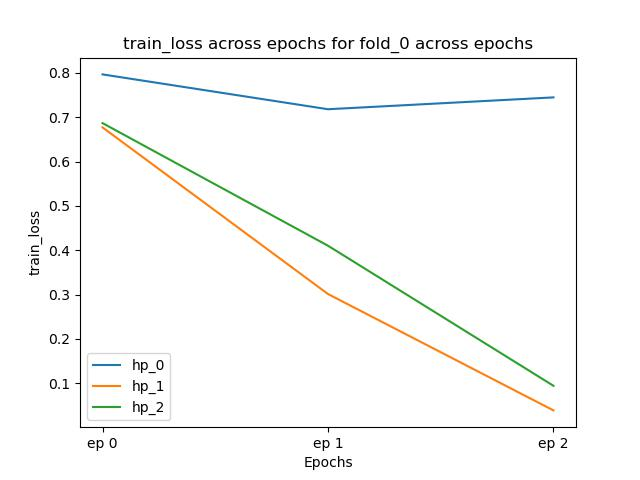
\includegraphics[scale = 0.75]{fold_0/train_loss}
\end{figure}
\subsection{test\_loss}
\begin{tabular}{lrrr}
\toprule
{} &   ep 0 &   ep 1 &   ep 2 \\
\midrule
hp\_0 &  0.757 &  0.705 &  0.703 \\
hp\_1 &  0.621 &  0.417 &  0.486 \\
hp\_2 &  0.599 &  0.512 &  0.500 \\
\bottomrule
\end{tabular}

\begin{figure}[H]
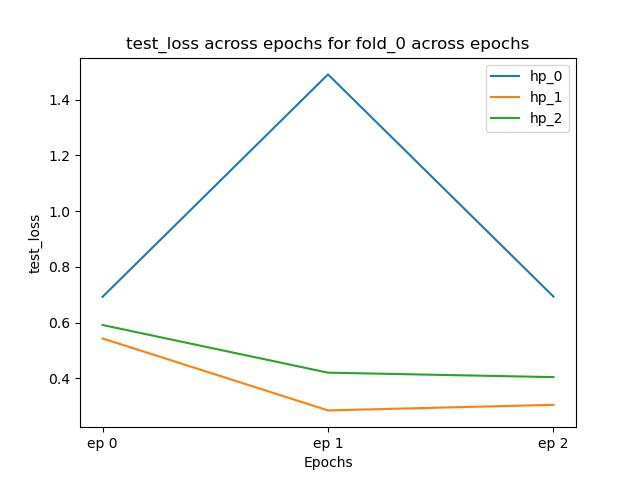
\includegraphics[scale = 0.75]{fold_0/test_loss}
\end{figure}
\subsection{accuracy\_score}
\begin{tabular}{lrrr}
\toprule
{} &   ep 0 &   ep 1 &   ep 2 \\
\midrule
hp\_0 &  0.496 &  0.496 &  0.496 \\
hp\_1 &  0.658 &  0.786 &  0.812 \\
hp\_2 &  0.709 &  0.778 &  0.812 \\
\bottomrule
\end{tabular}

\begin{figure}[H]
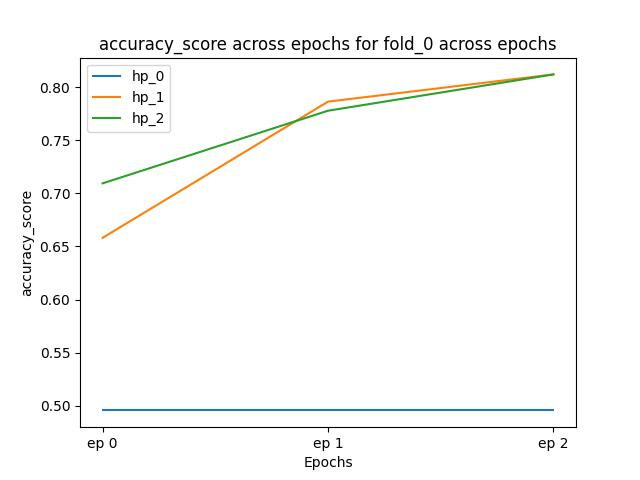
\includegraphics[scale = 0.75]{fold_0/accuracy_score}
\end{figure}
\subsection{f1\_score}
\begin{tabular}{lrrr}
\toprule
{} &   ep 0 &   ep 1 &   ep 2 \\
\midrule
hp\_0 &  0.663 &  0.663 &  0.663 \\
hp\_1 &  0.733 &  0.809 &  0.828 \\
hp\_2 &  0.754 &  0.797 &  0.823 \\
\bottomrule
\end{tabular}

\begin{figure}[H]
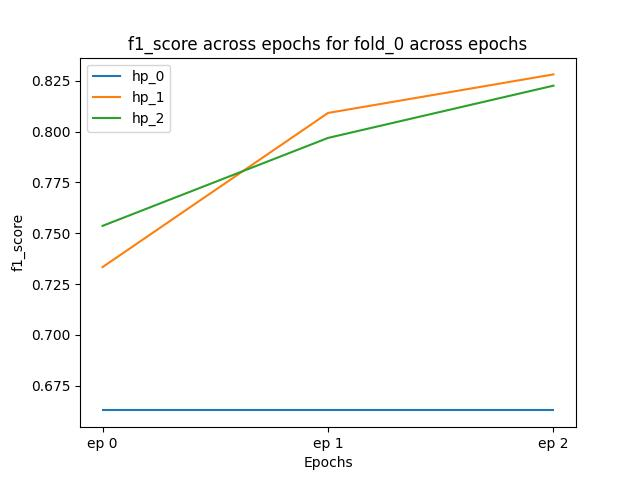
\includegraphics[scale = 0.75]{fold_0/f1_score}
\end{figure}
\subsection{precision\_score}
\begin{tabular}{lrrr}
\toprule
{} &   ep 0 &   ep 1 &   ep 2 \\
\midrule
hp\_0 &  0.496 &  0.496 &  0.496 \\
hp\_1 &  0.598 &  0.726 &  0.757 \\
hp\_2 &  0.650 &  0.729 &  0.773 \\
\bottomrule
\end{tabular}

\begin{figure}[H]
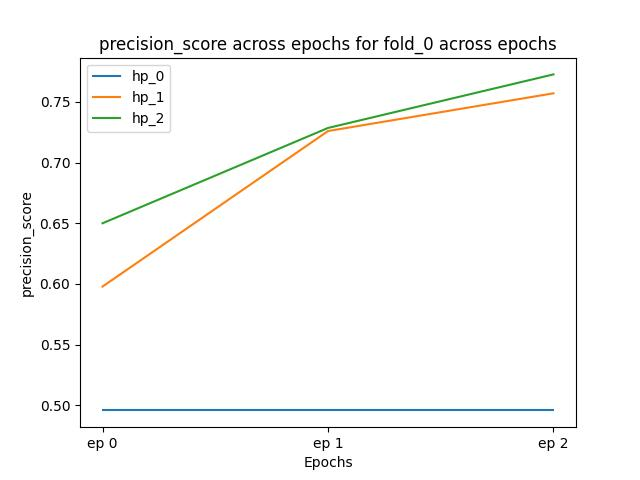
\includegraphics[scale = 0.75]{fold_0/precision_score}
\end{figure}
\subsection{matthews\_corrcoef}
\begin{tabular}{lrrr}
\toprule
{} &   ep 0 &   ep 1 &   ep 2 \\
\midrule
hp\_0 &  0.000 &  0.000 &  0.000 \\
hp\_1 &  0.392 &  0.593 &  0.638 \\
hp\_2 &  0.454 &  0.568 &  0.630 \\
\bottomrule
\end{tabular}

\begin{figure}[H]
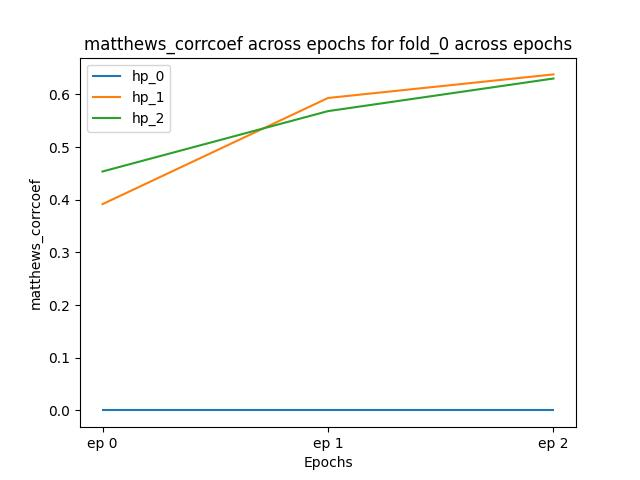
\includegraphics[scale = 0.75]{fold_0/matthews_corrcoef}
\end{figure}
\subsection{recall\_score}
\begin{tabular}{lrrr}
\toprule
{} &   ep 0 &   ep 1 &   ep 2 \\
\midrule
hp\_0 &  1.000 &  1.000 &  1.000 \\
hp\_1 &  0.948 &  0.914 &  0.914 \\
hp\_2 &  0.897 &  0.879 &  0.879 \\
\bottomrule
\end{tabular}

\begin{figure}[H]
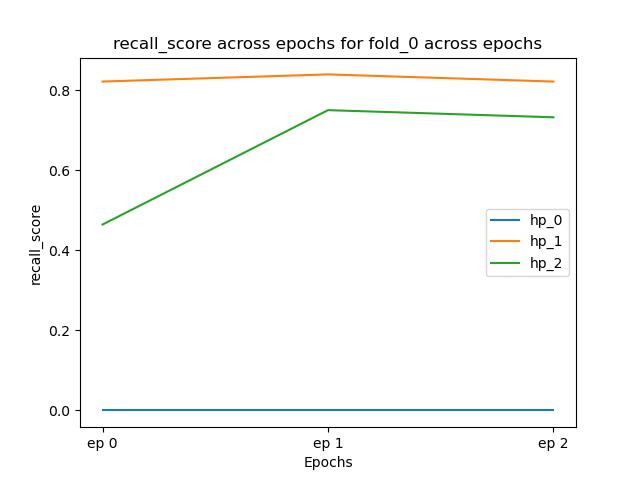
\includegraphics[scale = 0.75]{fold_0/recall_score}
\end{figure}
\section{fold\_1}
\subsection{train\_loss}
\begin{tabular}{lrrr}
\toprule
{} &   ep 0 &   ep 1 &   ep 2 \\
\midrule
hp\_0 &  0.687 &  0.552 &  0.147 \\
hp\_1 &  0.644 &  0.176 &  0.015 \\
hp\_2 &  0.658 &  0.380 &  0.073 \\
\bottomrule
\end{tabular}

\begin{figure}[H]
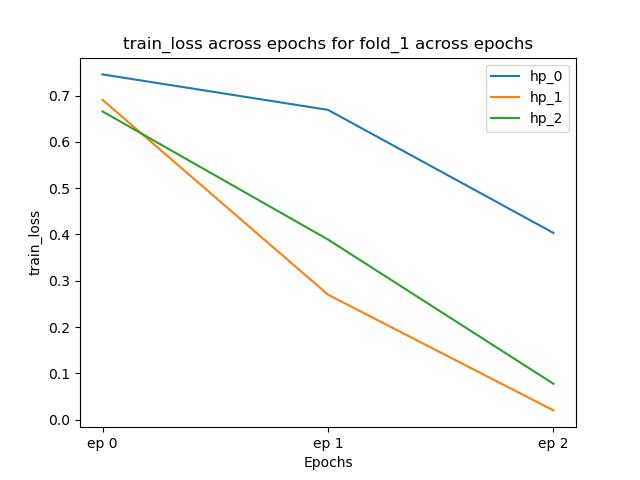
\includegraphics[scale = 0.75]{fold_1/train_loss}
\end{figure}
\subsection{test\_loss}
\begin{tabular}{lrrr}
\toprule
{} &   ep 0 &   ep 1 &   ep 2 \\
\midrule
hp\_0 &  0.596 &  0.507 &  0.525 \\
hp\_1 &  0.542 &  0.418 &  0.534 \\
hp\_2 &  0.621 &  0.444 &  0.437 \\
\bottomrule
\end{tabular}

\begin{figure}[H]
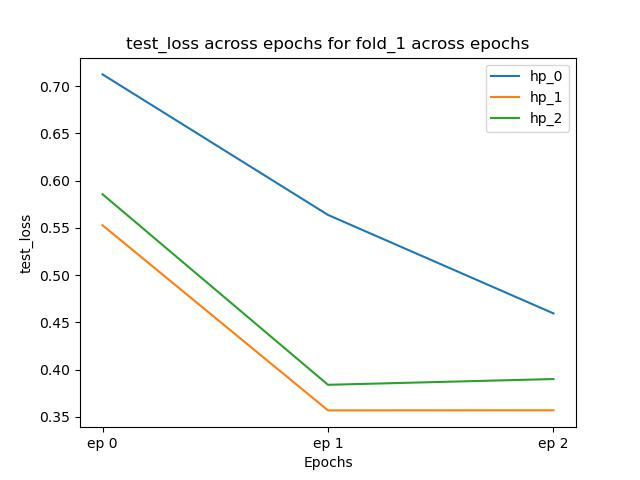
\includegraphics[scale = 0.75]{fold_1/test_loss}
\end{figure}
\subsection{accuracy\_score}
\begin{tabular}{lrrr}
\toprule
{} &   ep 0 &   ep 1 &   ep 2 \\
\midrule
hp\_0 &  0.716 &  0.819 &  0.853 \\
hp\_1 &  0.776 &  0.784 &  0.793 \\
hp\_2 &  0.638 &  0.767 &  0.793 \\
\bottomrule
\end{tabular}

\begin{figure}[H]
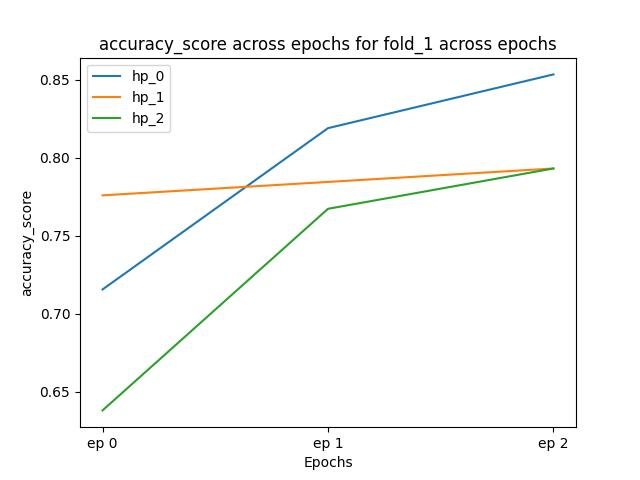
\includegraphics[scale = 0.75]{fold_1/accuracy_score}
\end{figure}
\subsection{f1\_score}
\begin{tabular}{lrrr}
\toprule
{} &   ep 0 &   ep 1 &   ep 2 \\
\midrule
hp\_0 &  0.713 &  0.811 &  0.864 \\
hp\_1 &  0.794 &  0.809 &  0.806 \\
hp\_2 &  0.650 &  0.777 &  0.797 \\
\bottomrule
\end{tabular}

\begin{figure}[H]
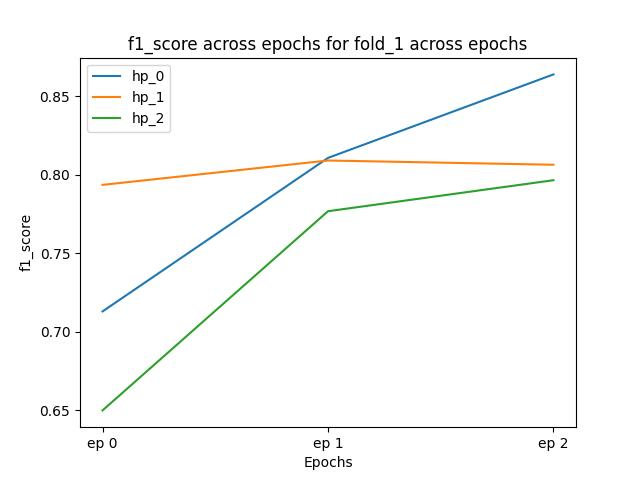
\includegraphics[scale = 0.75]{fold_1/f1_score}
\end{figure}
\subsection{precision\_score}
\begin{tabular}{lrrr}
\toprule
{} &   ep 0 &   ep 1 &   ep 2 \\
\midrule
hp\_0 &  0.745 &  0.882 &  0.831 \\
hp\_1 &  0.758 &  0.746 &  0.781 \\
hp\_2 &  0.650 &  0.770 &  0.810 \\
\bottomrule
\end{tabular}

\begin{figure}[H]
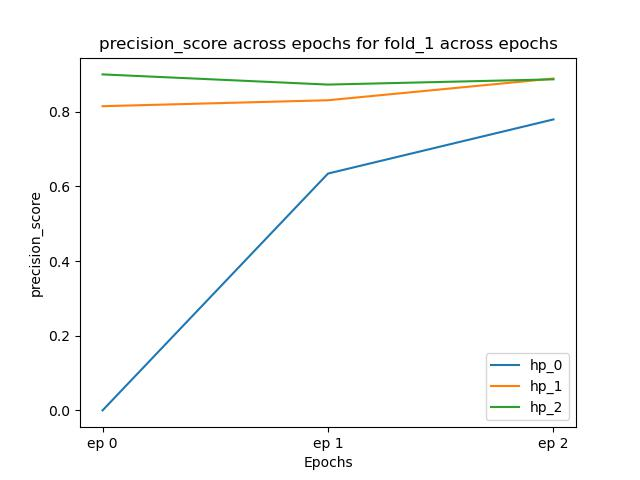
\includegraphics[scale = 0.75]{fold_1/precision_score}
\end{figure}
\subsection{matthews\_corrcoef}
\begin{tabular}{lrrr}
\toprule
{} &   ep 0 &   ep 1 &   ep 2 \\
\midrule
hp\_0 &  0.434 &  0.647 &  0.708 \\
hp\_1 &  0.553 &  0.576 &  0.586 \\
hp\_2 &  0.275 &  0.534 &  0.587 \\
\bottomrule
\end{tabular}

\begin{figure}[H]
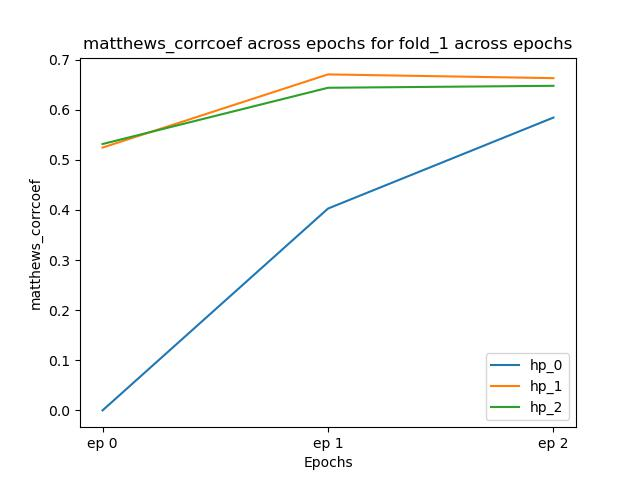
\includegraphics[scale = 0.75]{fold_1/matthews_corrcoef}
\end{figure}
\subsection{recall\_score}
\begin{tabular}{lrrr}
\toprule
{} &   ep 0 &   ep 1 &   ep 2 \\
\midrule
hp\_0 &  0.683 &  0.750 &  0.900 \\
hp\_1 &  0.833 &  0.883 &  0.833 \\
hp\_2 &  0.650 &  0.783 &  0.783 \\
\bottomrule
\end{tabular}

\begin{figure}[H]
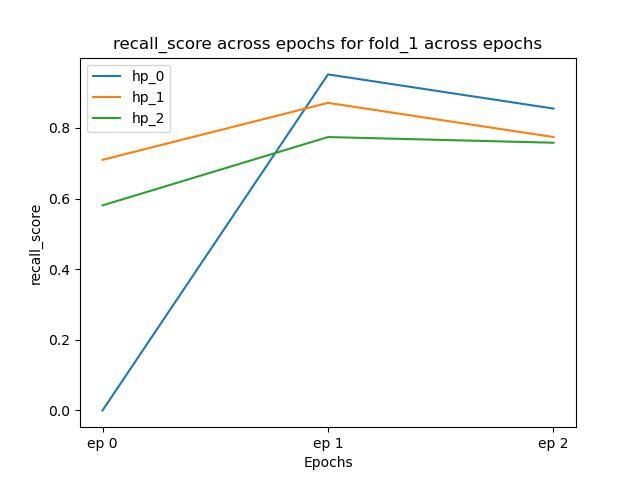
\includegraphics[scale = 0.75]{fold_1/recall_score}
\end{figure}
\section{fold\_2}
\subsection{train\_loss}
\begin{tabular}{lrrr}
\toprule
{} &   ep 0 &   ep 1 &   ep 2 \\
\midrule
hp\_0 &  0.795 &  0.688 &  0.420 \\
hp\_1 &  0.717 &  0.317 &  0.035 \\
hp\_2 &  0.715 &  0.508 &  0.116 \\
\bottomrule
\end{tabular}

\begin{figure}[H]
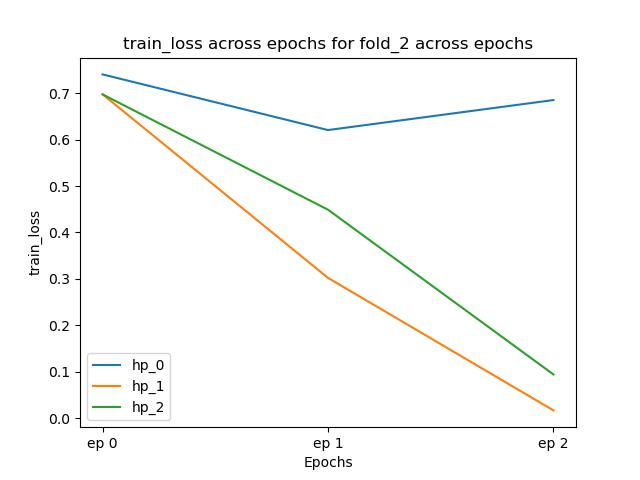
\includegraphics[scale = 0.75]{fold_2/train_loss}
\end{figure}
\subsection{test\_loss}
\begin{tabular}{lrrr}
\toprule
{} &   ep 0 &   ep 1 &   ep 2 \\
\midrule
hp\_0 &  0.704 &  0.712 &  0.666 \\
hp\_1 &  0.616 &  0.328 &  0.256 \\
hp\_2 &  0.634 &  0.455 &  0.331 \\
\bottomrule
\end{tabular}

\begin{figure}[H]
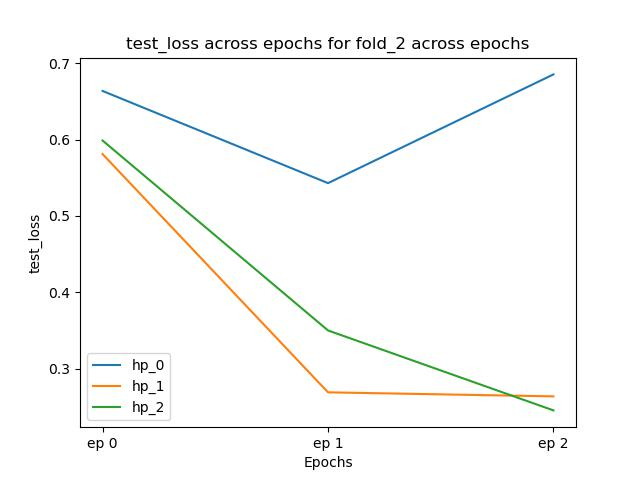
\includegraphics[scale = 0.75]{fold_2/test_loss}
\end{figure}
\subsection{accuracy\_score}
\begin{tabular}{lrrr}
\toprule
{} &   ep 0 &   ep 1 &   ep 2 \\
\midrule
hp\_0 &  0.414 &  0.414 &  0.672 \\
hp\_1 &  0.733 &  0.828 &  0.888 \\
hp\_2 &  0.698 &  0.802 &  0.845 \\
\bottomrule
\end{tabular}

\begin{figure}[H]
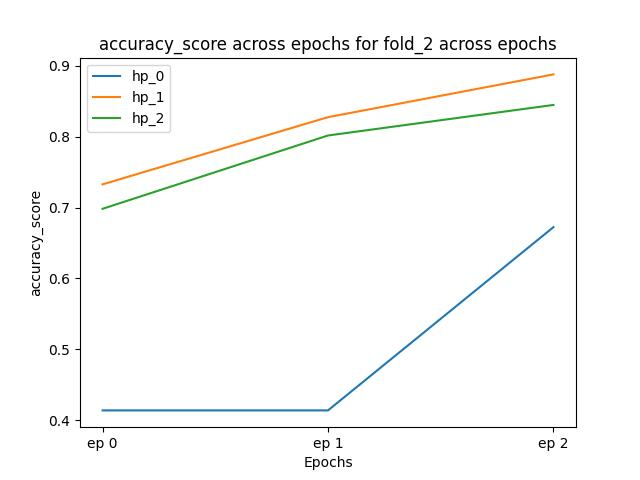
\includegraphics[scale = 0.75]{fold_2/accuracy_score}
\end{figure}
\subsection{f1\_score}
\begin{tabular}{lrrr}
\toprule
{} &   ep 0 &   ep 1 &   ep 2 \\
\midrule
hp\_0 &  0.585 &  0.585 &  0.345 \\
hp\_1 &  0.739 &  0.796 &  0.851 \\
hp\_2 &  0.624 &  0.793 &  0.804 \\
\bottomrule
\end{tabular}

\begin{figure}[H]
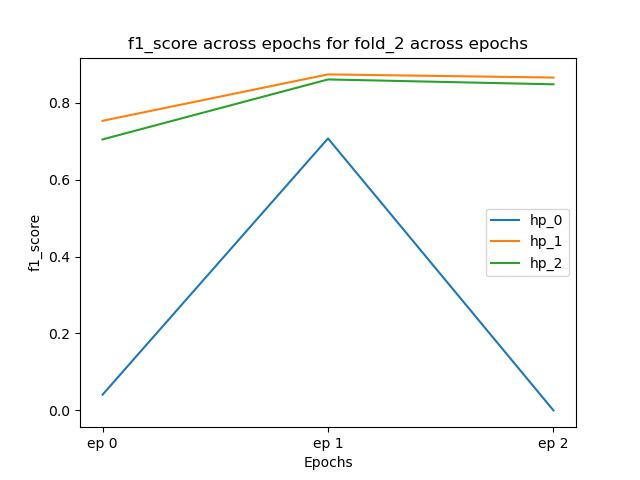
\includegraphics[scale = 0.75]{fold_2/f1_score}
\end{figure}
\subsection{precision\_score}
\begin{tabular}{lrrr}
\toprule
{} &   ep 0 &   ep 1 &   ep 2 \\
\midrule
hp\_0 &  0.414 &  0.414 &  1.000 \\
hp\_1 &  0.620 &  0.780 &  0.949 \\
hp\_2 &  0.644 &  0.698 &  0.841 \\
\bottomrule
\end{tabular}

\begin{figure}[H]
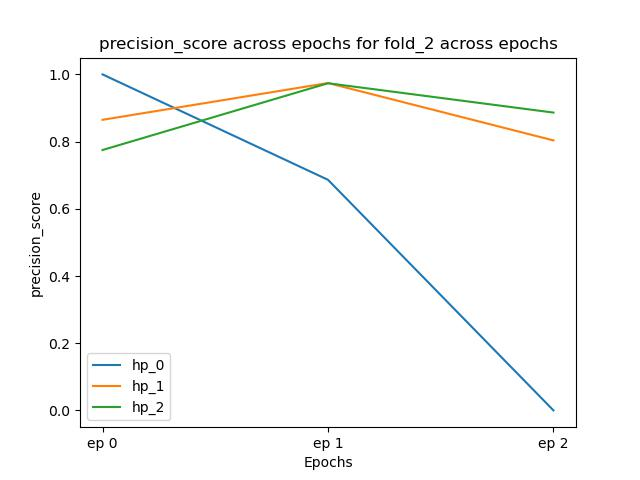
\includegraphics[scale = 0.75]{fold_2/precision_score}
\end{figure}
\subsection{matthews\_corrcoef}
\begin{tabular}{lrrr}
\toprule
{} &   ep 0 &   ep 1 &   ep 2 \\
\midrule
hp\_0 &  0.000 &  0.000 &  0.366 \\
hp\_1 &  0.525 &  0.647 &  0.773 \\
hp\_2 &  0.373 &  0.630 &  0.678 \\
\bottomrule
\end{tabular}

\begin{figure}[H]
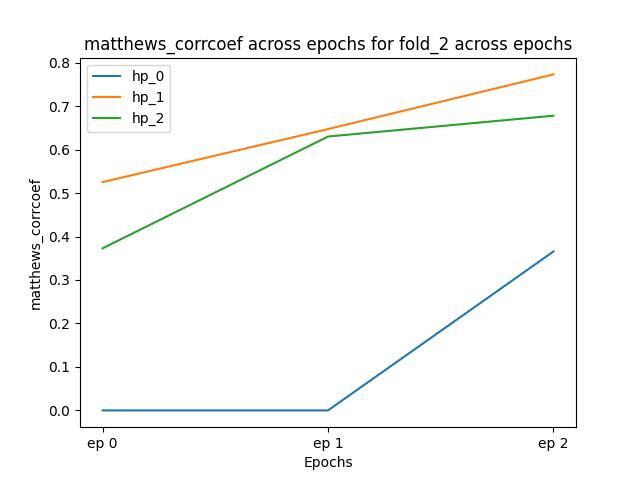
\includegraphics[scale = 0.75]{fold_2/matthews_corrcoef}
\end{figure}
\subsection{recall\_score}
\begin{tabular}{lrrr}
\toprule
{} &   ep 0 &   ep 1 &   ep 2 \\
\midrule
hp\_0 &  1.000 &  1.000 &  0.208 \\
hp\_1 &  0.917 &  0.812 &  0.771 \\
hp\_2 &  0.604 &  0.917 &  0.771 \\
\bottomrule
\end{tabular}

\begin{figure}[H]
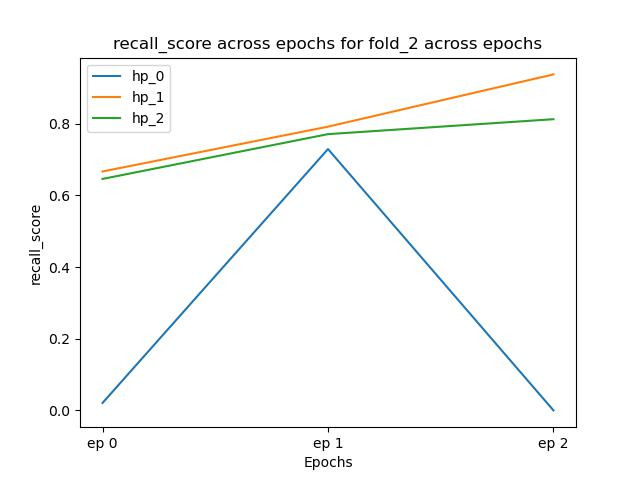
\includegraphics[scale = 0.75]{fold_2/recall_score}
\end{figure}
\end{document}
